\begin{subfigure}[t]{\textwidth}
  \centering
  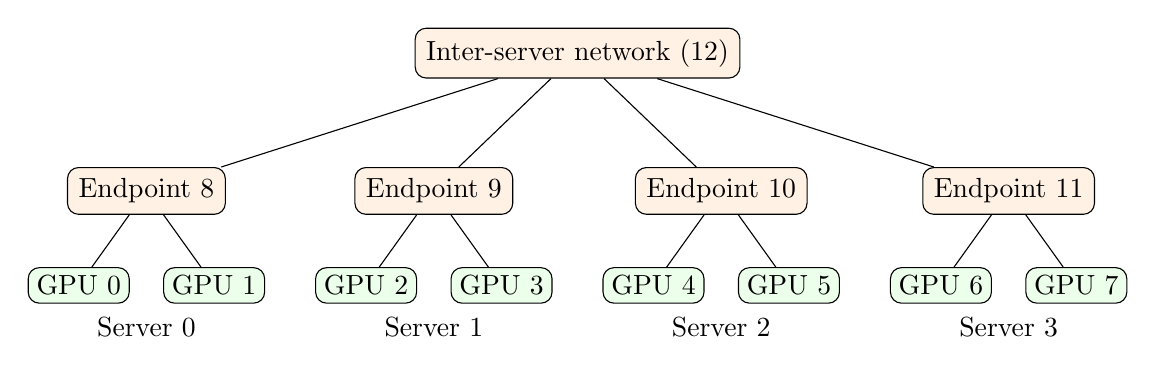
\begin{tikzpicture}[x=1cm,y=1cm,
    endpoint/.style={draw, rounded corners, fill=orange!10, inner sep=4pt},
    gpu/.style={draw, rounded corners, fill=green!8, inner sep=3pt}]
    \node[endpoint] (fabric) at (7.125,3.25) {Inter-server network (12)};
    \foreach \server in {0,...,3} {
      \pgfmathtruncatemacro{\firstgpu}{2*\server}
      \pgfmathtruncatemacro{\secondgpu}{2*\server+1}
      \pgfmathtruncatemacro{\endpointid}{8+\server}
      \begin{scope}[shift={({1.65+3.65*\server},0)}]
        \node[endpoint] (endpoint-\server) at (0,1.5) {Endpoint \endpointid};
        \node[gpu] (first) at (-0.86,0.3) {GPU \firstgpu};
        \node[gpu] (second) at (0.86,0.3) {GPU \secondgpu};
        \draw (endpoint-\server) -- (first);
        \draw (endpoint-\server) -- (second);
        \node at (0,-0.23) {Server \server};
      \end{scope}
      \draw (fabric) -- (endpoint-\server);
    }
  \end{tikzpicture}
  \caption{Two-tier topology. GPU-to-endpoint links have $C_e=2$;
  endpoint-to-network links have $C_e=1$.}
\end{subfigure}\par\medskip
\begin{subfigure}[t]{\textwidth}
  \centering
  \begin{tikzpicture}[
    rank/.style={draw, rounded corners, fill=green!8, minimum width=0.85cm},
    transfer/.style={-{Stealth}, semithick},
    expert/.style={font=\small, fill=white, inner sep=1.5pt}]
    \node[rank] (before7) at (0,0) {R7};
    \node[rank] (before1) at (2.7,0) {R1};
    \node[rank] (before5) at (5.5,1.2) {R5};
    \node[rank] (before6) at (5.5,0) {R6};
    \node[rank] (before0) at (5.5,-1.2) {R0};
    \node[rank] (before3) at (8.3,1.2) {R3};
    \node[rank] (before4) at (8.3,-1.2) {R4};
    \node[rank] (before2) at (11.4,0) {R2};
    \foreach \src/\dst/\expert in {7/1/5,1/5/7,1/6/8,1/0/1,5/3/3,6/2/4,0/4/6,4/2/2}
      \draw[transfer] (before\src) -- node[expert,above] {E\expert} (before\dst);
  \end{tikzpicture}
  \caption{All migrations issued together.}
\end{subfigure}\par\medskip
\begin{subfigure}[t]{\textwidth}
  \centering
  \begin{tikzpicture}[
    rank/.style={draw, rounded corners, fill=green!8, minimum width=0.85cm},
    transfer/.style={-{Stealth}, semithick},
    expert/.style={font=\small, inner sep=1pt}]
    \foreach \batch in {0,1,2} {
      \begin{scope}[shift={({5.05*\batch},0)}]
        \draw[rounded corners, fill=blue!4] (-0.55,-0.55) rectangle (4.25,2);
        \node[font=\bfseries] at (1.85,1.63) {Batch \batch};
      \end{scope}
    }
    \node[rank] (batch-zero-one) at (0,0.52) {R1};
    \node[rank] (batch-zero-zero) at (1.8,1.03) {R0};
    \node[rank] (batch-zero-six) at (1.8,0) {R6};
    \node[rank] (batch-zero-two) at (3.65,0) {R2};
    \draw[transfer] (batch-zero-one) -- node[expert,above] {E1} (batch-zero-zero);
    \draw[transfer] (batch-zero-one) -- node[expert,below] {E8} (batch-zero-six);
    \draw[transfer] (batch-zero-six) -- node[expert,above] {E4} (batch-zero-two);
    \begin{scope}[shift={(5.05,0)}]
      \foreach \rankid [count=\index from 0] in {7,1,5,3}
        \node[rank] (batch-one-\rankid) at ({1.22*\index},0.52) {R\rankid};
      \foreach \src/\dst/\expert in {7/1/5,1/5/7,5/3/3}
        \draw[transfer] (batch-one-\src) -- node[expert,above=6pt] {E\expert} (batch-one-\dst);
    \end{scope}
    \begin{scope}[shift={(10.1,0)}]
      \foreach \rankid [count=\index from 0] in {0,4,2}
        \node[rank] (batch-two-\rankid) at ({0.1+1.75*\index},0.52) {R\rankid};
      \foreach \src/\dst/\expert in {0/4/6,4/2/2}
        \draw[transfer] (batch-two-\src) -- node[expert,above] {E\expert} (batch-two-\dst);
    \end{scope}
  \end{tikzpicture}
  \caption{ILP schedule: the three batches execute from left to right.}
\end{subfigure}
